\documentclass[12pt]{article}  % 官方要求字号不小于 12 号,此处选择 12 号字体
% \linespread{1.1}
% \bibliographystyle{plain}
\usepackage[2422020]{easymcm} 
\problem{A} 
\usepackage{times}
\usepackage{pdfpages}
\usepackage{longtable}
\usepackage{tabu}
\usepackage{threeparttable}
\usepackage[ruled,linesnumbered]{algorithm2e}
\usepackage{algpseudocode}
\usepackage{listings}
\usepackage{paralist}
\usepackage{array}
\graphicspath{{img/}}         
 \let\itemize\compactitem
 \let\enditemize\endcompactitem
\newcommand{\upcite}[1]{\textsuperscript{\textsuperscript{\cite{#1}}}}
\title{Lamprey Gender Control: Interactions with Ecosystem
}  % 标题
% 如需要修改题头(默认为 MCM/ICM),请使用以下命令(此处修改为 MCM)
%\renewcommand{\contest}{MCM}

 %文档开始
\begin{document}

% 此处填写摘要内容
\begin{abstract}
  In everyday life, it seems absurd to us to change genders.  But there are creatures that disrupt what we know about gender transition.  Lampreys are a good example of a population whose sex ratio can vary according to the external environment: the sex of lampreys is determined by the growth rate of their larvae, the male sex ratio of lampreys is higher when the environment is poor, and the male sex ratio tends to be 1:1 when the environment is good.  This is not surprising in nature, and this condition is called \textbf{adaptive sex ratio variation} in biology.  This adaptive sex ratio variation is of great significance for our study of local species diversity.

	To begin with, we established the \textbf{Internal Relations Model}. Firstly, we determine the relationship between biological length and time base on the \textbf{Von Bertalanffy Growth Model}. Then, the \textbf{Sex Determination Model }is established according to the logical model. Finally, the \textbf{Population Growth Model} in a specific area was established.   In order to obtain the growth rate parameters $ k$ and logistic regression parameters $\beta_{0}$, $\beta_{1}$, we use \textbf{nonlinear least square method }to fit and get the corresponding optimal parameters.

On this basis, we established the \textbf{Interaction Model} to simulate the interaction between lampreys population and external environment. At the same time, we also innovatively proposed the concept of \textbf{interaction degree} to quantitatively measure the interaction between species and external environment in each area,and the parameters of\textbf{ Lotka-Volterra Model} are also reasonably estimated.

Based on the Internal Relations Model and Interaction Model, we further established a \textbf{Host-Parasite Model} to consider the effects of parasites on lampreys populations.At this point, the model has been established and the important parameters have been reasonably estimated,and the problems in the Requirement have been solved as follows:


\begin{itemize}
	\setlength{\parsep}{0ex} %段落间距
	\setlength{\topsep}{2ex} %列表到上下文的垂直距离
	\setlength{\itemsep}{1ex} %条目间距
	\item According to the calculation and comparison of the interaction degree, when the male proportion of lampreys population is between \textbf{48$\%$ and 63$\%$,} the interaction degree between lampreys population and the ecosystem is malignant; when the male proportion of lampreys population is higher than \textbf{63$\%$}, the interaction degree between lampreys population and the ecosystem is   benign.
	\item In harsh environments, the \textbf{advantage }of lampreys populations is to control their growth rate, sex ratio, and overall size to stabilize prey numbers and male to female ratios. However, even in favorable circumstances, incorrect sex ratios can hinder population recovery.
	\item By calculating the interaction degree between lampreys population and the ecosystem, and taking the data of \textbf{the Great Lakes} from 2016 to 2021, we obtained the interaction degree value of lampreys as \textbf{85.846} when the sex ratio is 70 percent,indicating that it is \textbf{not conducive} to the stability of the ecosystem.At the same time, when the sex ratio is 50 $\%$, it is malignant coupling to the environment.
	\item Based on the Host-Parasite Model, we found that lampreys\textbf{ compete with} other species represented by parasites, so such an ecosystem \textbf{does not provide an advantage} to other species
\end{itemize}

Finally, the sensitivity of the model is analyzed comprehensively.The model performed well.

    % 美赛论文中无需注明关键字。若您一定要使用,
    % 请将以下两行的注释号 '%' 去除,以使其生效
    \vspace{5pt}  %mm	毫米	1 mm = 2.845 pt   pt 点	1 pt = 0.351 mm
    \textbf{Keywords}: Lampreys; Internal Relations Model; Interaction Model;  Host-Parasite Model; Sensitivity Analysis ; Interaction Degree

\end{abstract}

\maketitle  % 生成 Summary Sheet

\tableofcontents  % 生成目录


% 正文开始
% Chapter 1: Introduction
\section{Introduction}

\subsection{Problem Background}
As a prime example of nature's mastery in gender flexibility, the lamprey demonstrates an adaptive sex that is responsive to its surrounding environment.   In ecosystems abundant with nourishment and resources, the sex ratio is basically maintained at 1:1.   Conversely, in environments characterized by limited resources, the male population thrives, embodying remarkable resilience.   Here's a captivating photo of a lamprey that truly encapsulates the enchantment of nature's transformative powers:
\begin{figure}[htbp]  %h此处,t页顶,b页底,p独立一页,浮动体出现的位置
\centering  %图表居中
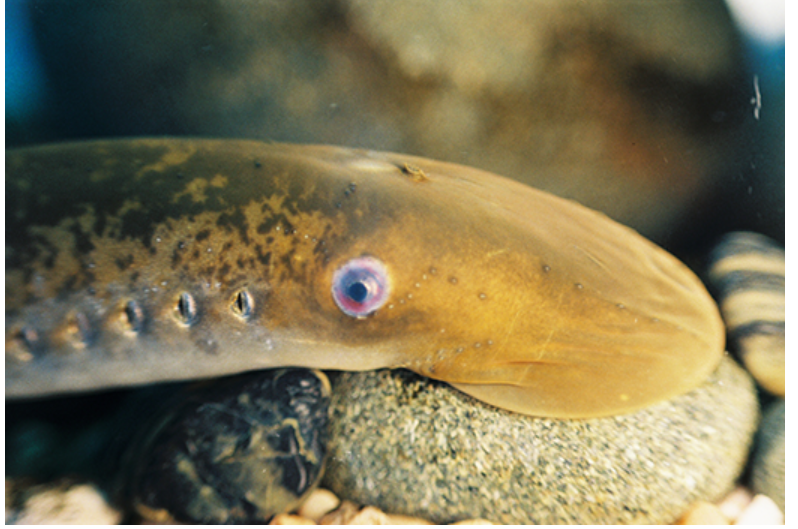
\includegraphics[width=.7\textwidth]{lamprey.png} %图片的名称或者路径之中有空格会出问题 
\caption{A Lamprey in River}
\label{fig:lamprey} % 图片标签,可以不写
\end{figure}

The picture above comes from the website \textbf{Great Lakes Fishery Commission}\upcite{1}.The natural world offers numerous examples of sex ratios adapting to environmental conditions.  For instance, certain lizard species demonstrate a preference for producing females in warmer environments and males in colder environments.  This adaptive variation in sex ratios is a result of local biodiversity and holds significant research value.

\subsection{Restatement of the Problem}
The study of species is an exceedingly intricate undertaking. By conducting thorough analysis and research on the contextual intricacies, in conjunction with the specific limitations provided, the restatement of the problem can be articulated as follows:
\begin{itemize}
\setlength{\parsep}{0ex} %段落间距
\setlength{\topsep}{2ex} %列表到上下文的垂直距离
\setlength{\itemsep}{1ex} %条目间距
\item Build a mathematical models to establish the effects of changing the sex ratio of lampreys in a population on the larger ecosystem.
\item Establish the strengths and weaknesses of lampreys populations.
\item Based on changes in the sex ratio of lampreys, explain the impact on ecosystem stability.
\item Determine whether ecosystems in which the sex ratio of lamprey populations is variable provide an advantage to other species in the ecosystem, such as parasites.
\end{itemize}
\subsection{Our Work}
In order to avoid complicated description, intuitively reflect our work process, the flow chart is shown in Figure 2:

\begin{figure}[htbp]  %h此处,t页顶,b页底,p独立一页,浮动体出现的位置
\centering  %图表居中
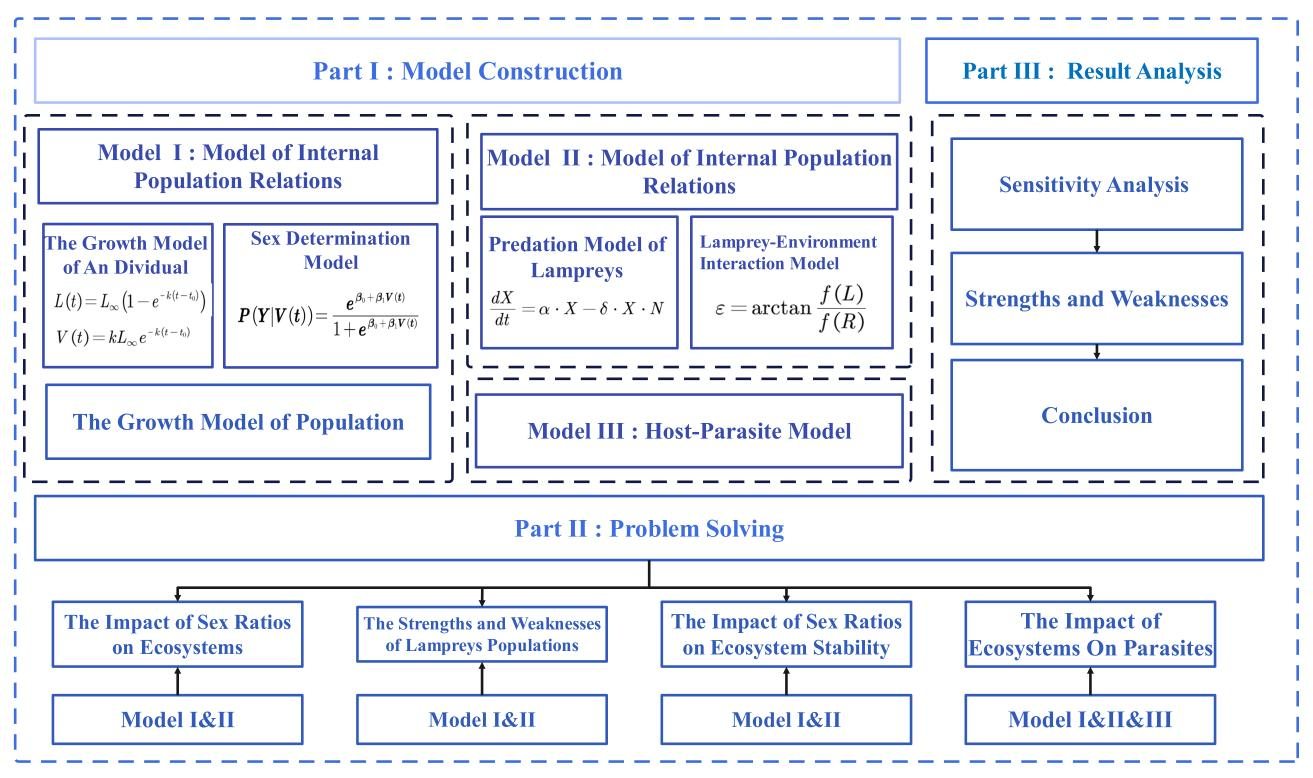
\includegraphics[width=1.\textwidth]{Flow_Chart.jpg} %图片的名称或者路径之中有空格会出问题 
\caption{Flow Chart of Our Work} % 图片标题 
\end{figure}
\vspace{-0.8cm}
\section{Assumptions and Explanations}
The complexity of real problems necessitates the initial formulation of reasonable assumptions in order to simplify the model, with each assumption being accompanied by a corresponding explanation:

\textbf{Assumption 1:}Only the influence of availability of food on lampreys is considered, and other factors such as temperature and atmosphere are ignored.

\textbf{Explanation:}In our model, the object of our study is mainly the availability of food, and the influence of other factors is small, so it can be ignored.


\textbf{Assumption 2:}In order to reduce competition for food resources, lampreys tend to be more evenly distributed in the areas where they live.

\textbf{Explanation:}The distribution of lampreys was uniform across the study area.

\textbf{Assumption 3:}The main source of sustenance for lampreys consists of fish.

\textbf{Explanation:}Lampreys prey on a wide range, the main source of food is fish, so the food source is assumed to be fish.

\textbf{Assumption 4:}The lampreys face no competition.

\textbf{Explanation:}Lampreys can prey on many animals because their wide range of prey gives them fewer competitors.


\textbf{Assumption 5:}The relationship between growth rate and food availability is a one-time function.

\textbf{Explanation:}The growth rate of lampreys exhibits a linear correlation with the food availability in their environment, as stated in \textbf{JIM HONE's}\upcite{2} paper.

In order to simplify the analysis of the various parts, some additional assumptions have been made. These assumptions will be discussed in due course.

\section{Notations}
The mathematical notations of significance utilized in this paper are enumerated in Table 1.
\vspace{-0.4cm}
\begin{table}[htbp]
\begin{center}
\caption{Notations used in this paper}
\begin{tabular}{c l c}
\toprule[2pt]
\textbf{Symbol}
&\textbf{Description}
&\textbf{Unit }
\\
\midrule
$L(t)$& The length of an individual organism at a certain time& mm \\
$L_{\infty}$& The maximum attainable length of an individual organism& mm\\
$k$& A positive parameter related to growth rate&/\\
$t_{0}$& The age at which an organism begins to grow &/\\
$V(t)$ & The rate of growth &mm/s\\
\vspace{5pt}%公式间有点挤,空一些
$\beta_{0},\beta_{1}$ & Logistic regression parameter&/\\
\vspace{3pt}
$N$ &The number of lampreys' population in a given area&/\\
$M$&The total number of males of a species&/\\
$F$&The total number of females of a species&/\\
$S$&The proportion of males in the population&/\\
$c_{i}$& The proportion of eggs that develop into males&/\\
$X$ & The total number of individuals in the prey population&/\\
$\varepsilon$& Interation Degree &/\\
$I$ & The number of parasites&/\\
$h$ & The natural mortality rate of parasites&/\\
$q$ & The ratio of the number of hosts infected by parasites to the total population&/\\
$J$ & The number of hosts&/\\
$c_{i}$ &  The proportion of eggs that develop into males&/\\
$\gamma$&  The parameter used to modify the equation&/\\ 
 $e_{i}$& The larval survival rate&/\\
 $\alpha$  & 	The natural growth rate of the prey population&/\\
 $\delta $& The percentage of the total prey that is hunted&/\\
\bottomrule[2pt]
\end{tabular}\label{tb:notation}
 \begin{tablenotes}
        \footnotesize
        \item[*] *The variables not listed here will be discussed in detail in each respective sectio. %此处加入注释*信息
      \end{tablenotes}
\end{center}
\end{table}
\vspace{-1.5cm}%在\end{table}下加一行\vspace{-1cm} 其中-1的作用是缩短与下方文字距离的 切记!必须是负数

\section{Model Preparation}
\subsection{Data Overview}
This problem lacks direct data, necessitating the acquisition of relevant data for our model construction.   A meticulous analysis of the issue highlights the need to gather comprehensive information on lampreys over an extended period, \textbf{encompassing growth rate, sex ratio, average length, and other pertinent factors}.   Consequently, we collected extensive data from 1997 to 2010 in \textbf{the Great Lakes }region.   Given the substantial volume of data involved, it is impractical to enumerate all aspects,hence visualizing the data proves advantageous.

\subsection{Data Collection}
The official website of \textbf{the Great Lakes Fishery Commission }\upcite{1}was accessed to retrieve a wealth of data on lampreys. Additionally, Table 2 presents other sources of data.

\begin{table}[htbp]
\begin{center}
\caption{Data and Database Websites}
\resizebox{\textwidth}{!}
{\begin{tabular}{c c}
\toprule[2pt]
\multicolumn{1}{m{5cm}}{\centering \textbf{Database Names}}
&\multicolumn{1}{m{10cm}}{\centering \textbf{Database Websites} }\\ %m后面是列宽
\midrule
Google Scholar & https://scholar.google.com/ \\
China National Knowledge Infrastructure& https://www.cnki.net/\\
WanFang Database& https://www.wanfangdata.com.cn/\\
\bottomrule[2pt]
\end{tabular}}
\end{center}
\end{table}
\vspace{-0.5cm}


\section{Model Establishment}
\subsection{Model I:Model of Internal Population Relations }
\subsubsection{The Growth Model of An Individual of A Species in A Given Area }
The following section presents a growth model for aquatic organisms in a specific geographical area. In this particular scenario, we define $L(t)$ as the length of an organism at time $ t$, and the growth of the organism's length can be accurately described by the \textbf{Von Bertalanffy growth function}, which is expressed as follows:
\begin{equation}
	L\left( t \right) =L_{\infty}\left( 1-e^{-k\left( t-t_0 \right)} \right) 
\end{equation}
where:
\begin{itemize}
	\setlength{\parsep}{0ex} %段落间距
	\setlength{\topsep}{2ex} %列表到上下文的垂直距离
	\setlength{\itemsep}{1ex} %条目间距
	\item $L_{\infty}$ is the maximum length that an individual can grow to.
	\item $t_{0}$ is the age at which an individual begins to grow.
	\item $k$ is a positive parameter of growth rate.
	\item $e$ is the base of the natural logarithm(It is equal to 2.71828).
\end{itemize}

The underlying assumption of this model is that the growth rate of an organism is directly proportional to the disparity between its maximum potential length and its current size, with a gradual deceleration in growth as it approaches its full maturity.  This concept aligns well with the observed growth patterns in numerous animal species, thus we employed this model to simulate the actual growth dynamics of lampreys.

The growth rate $V(t)$ of lampreys at a specific moment can also be derived at this juncture :
\begin{equation}
	V(t)=\frac{dL\left( t \right)}{dt}=kL_{\infty}e^{-k\left( t-t_0 \right)}
\end{equation}
\begin{figure}[H]
	\centering    
	\subfigure[The Growth Model $L(t)$]{				% 图片1([]内为子图标题)						
		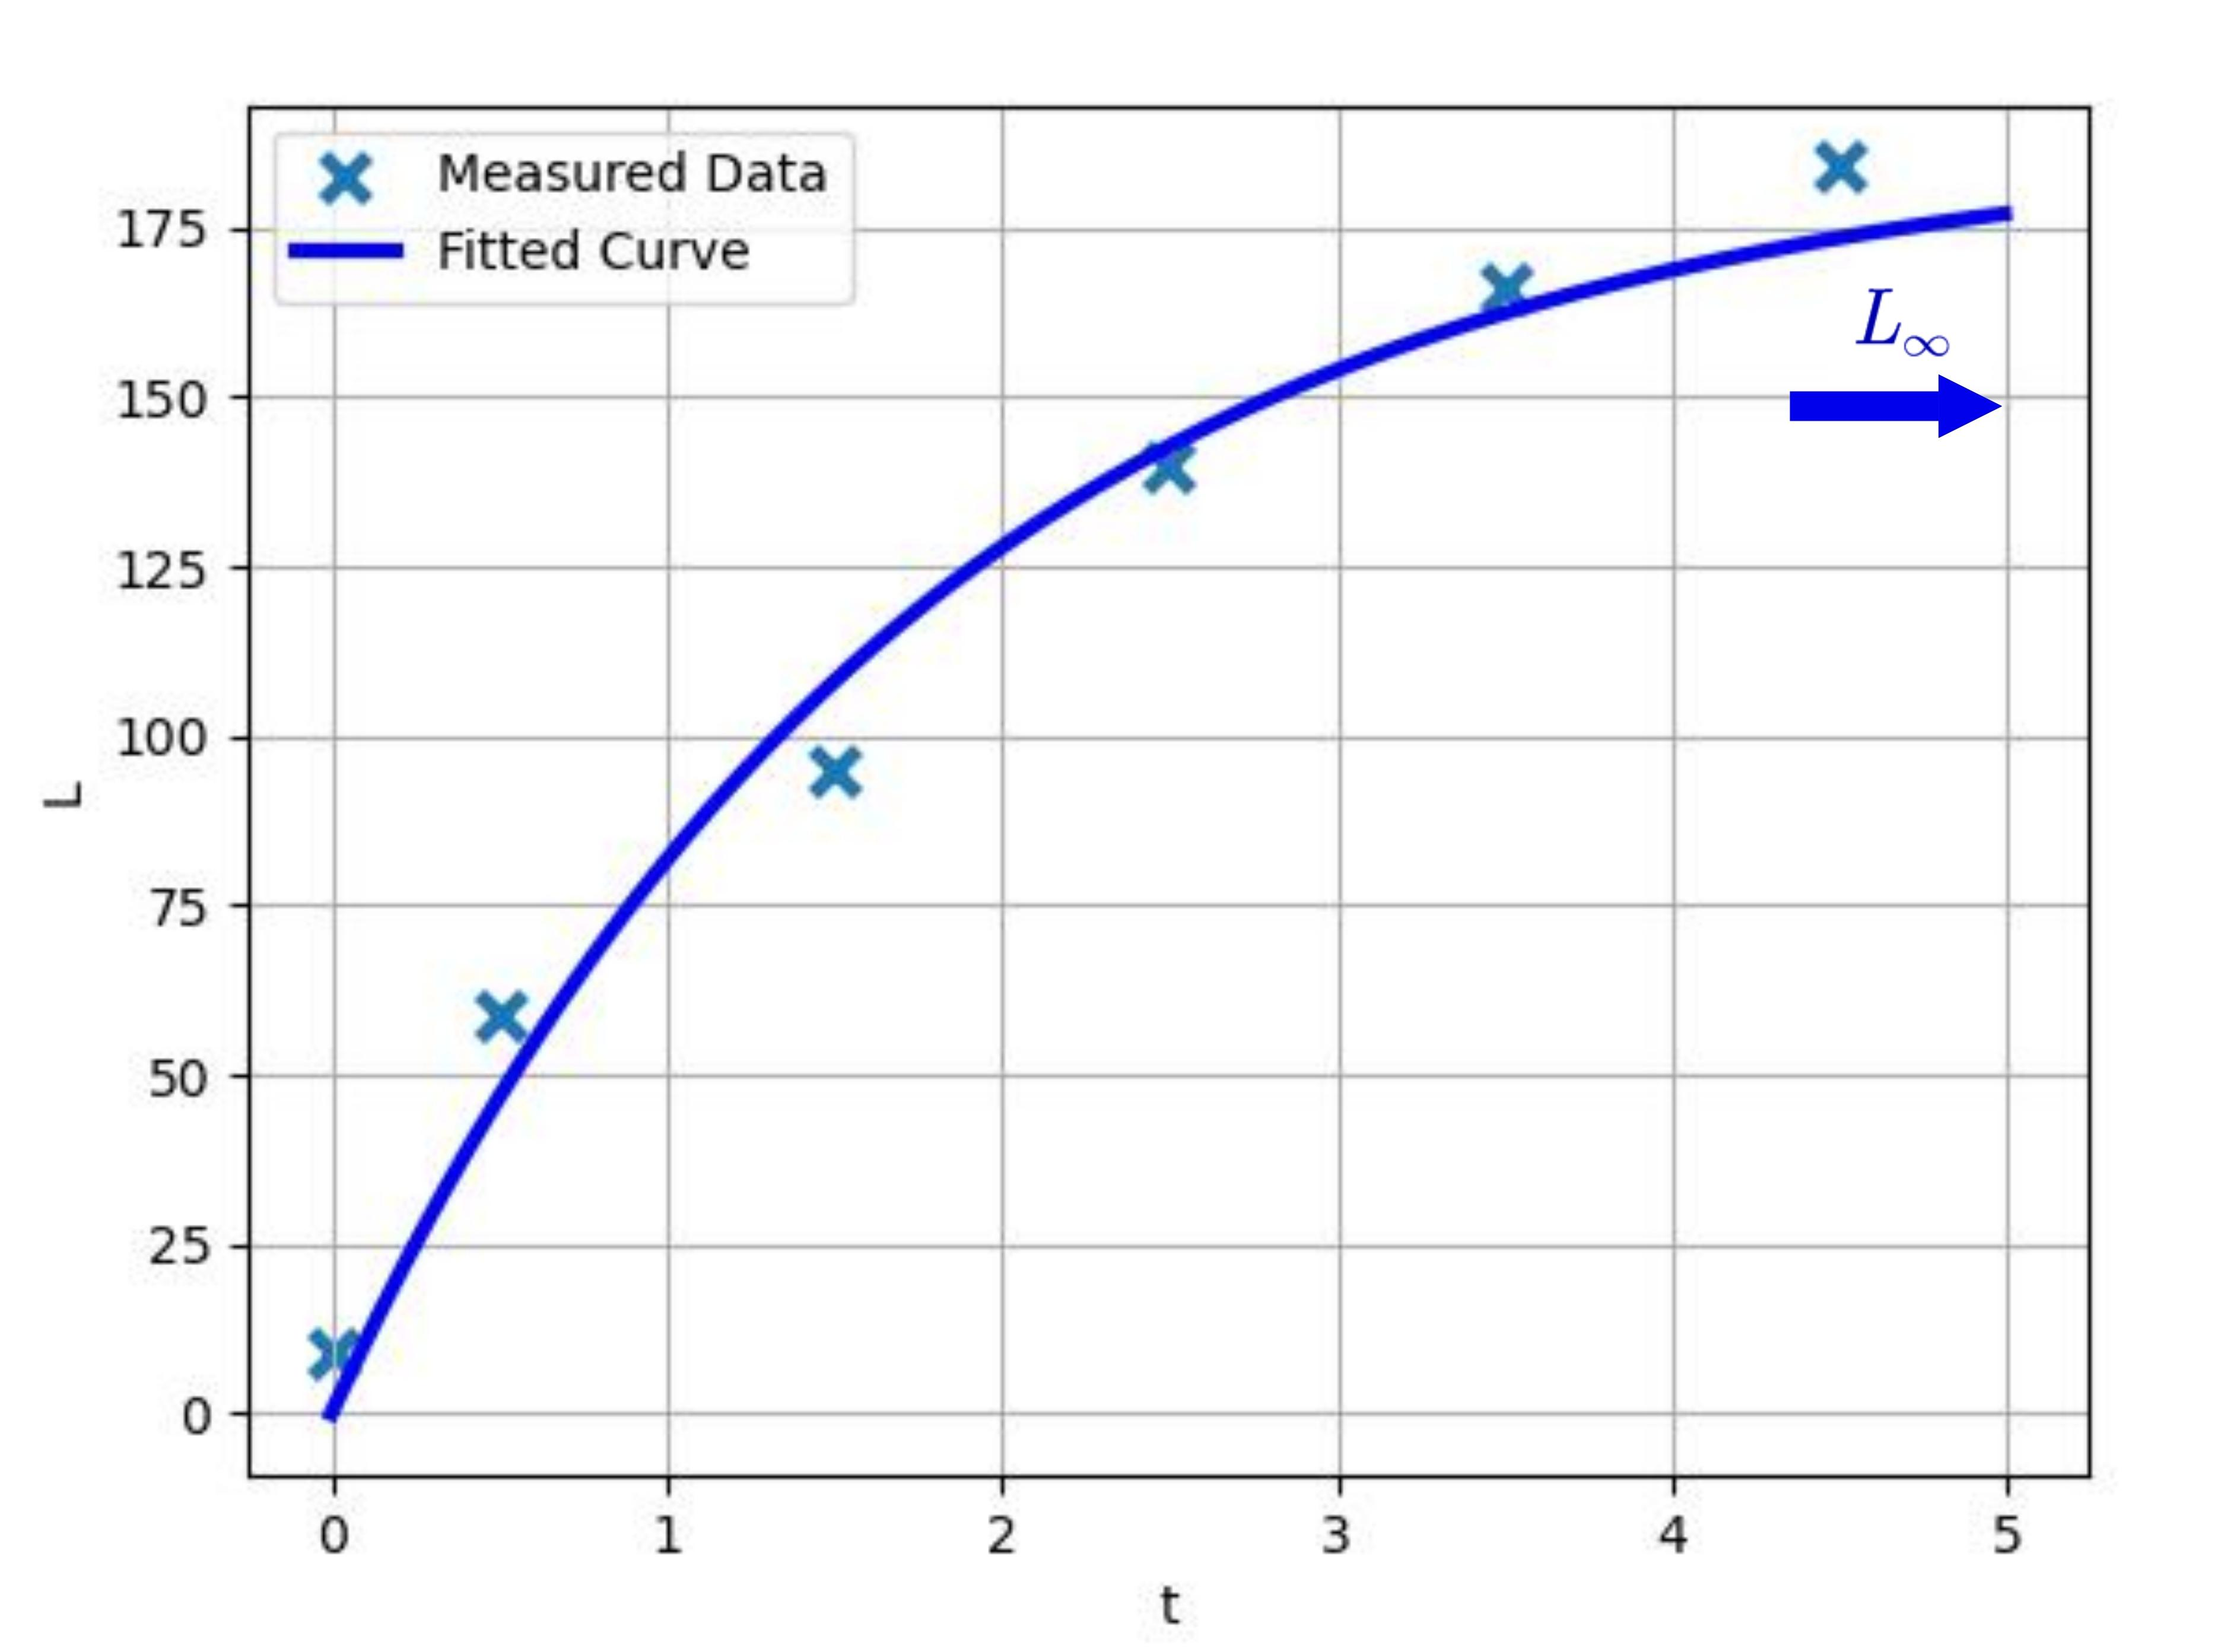
\includegraphics[width=0.43\textwidth]{生长模型.jpg}}			  % 子图1的图片宽度 不能空行
	\subfigure[The Growth Rate $V(t)$]{				% 图片2
		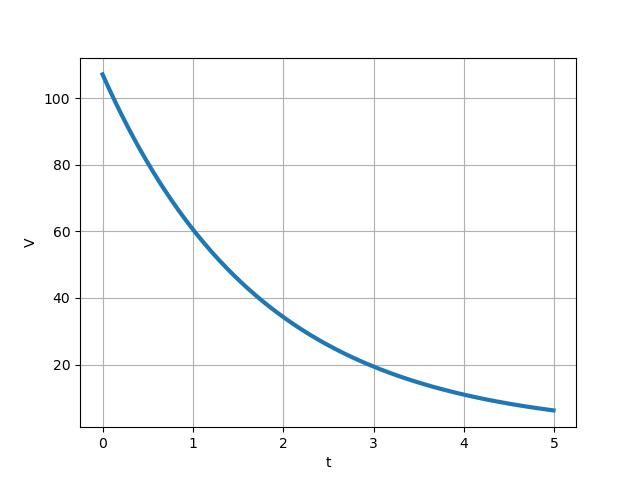
\includegraphics[width=0.45\textwidth]{发育速度 (1).jpg}}
	
	\caption{Model and Data Fitting} % 图片标题 
\end{figure}

The image above depicts how we employ the data we've amassed to tailor our model.
\subsubsection{Sex Determination Model }

\begin{equation}
	P\left( \left. Y=1 \right|V\left( t \right) \right) =\frac{e^{\beta _0+\beta _1\cdot V\left( t \right)}}{1+e^{\beta _0+\beta _1\cdot V\left( t \right)}}
\end{equation}
where:
\begin{itemize}
	\setlength{\parsep}{0ex} %段落间距
	\setlength{\topsep}{2ex} %列表到上下文的垂直距离
	\setlength{\itemsep}{1ex} %条目间距
	\item $P\left( \left. Y=1 \right|V\left( t \right) \right)$ is the probability function representing the relationship between the presence of females in lampreys and the growth rate of lampreys.
	\item $\beta_{0}$ and $\beta_{1}$ are logistic regression parameters.
\end{itemize}

The current understanding of the relationship between sex ratio and growth rate has led us to recognize that the growth rate of lampreys is also influenced by the food availability in their environment.  Therefore, it is imperative for us to further investigate the correlation between the growth rate $V(t)$ of lampreys and their environmental food resources.

The growth rate of lampreys $V(t)$ exhibits a linear correlation with the food availability in their environment, as stated in \textbf{JIM HONE's}\upcite{2} paper, the specific expression is as follows:
\begin{equation}
	V(t)=a+b\cdot R
\end{equation}

where:
\begin{itemize}
	\setlength{\parsep}{0ex} %段落间距
	\setlength{\topsep}{2ex} %列表到上下文的垂直距离
	\setlength{\itemsep}{1ex} %条目间距
	\item $a$ and $b$ are are constants.
	\item $R$  is the level of food availability.
\end{itemize}
\begin{figure}[H]
	\centering    
	\subfigure[$P\left( \left. Y=1 \right|V\left( t \right) \right) $]{				% 图片1([]内为子图标题)						
		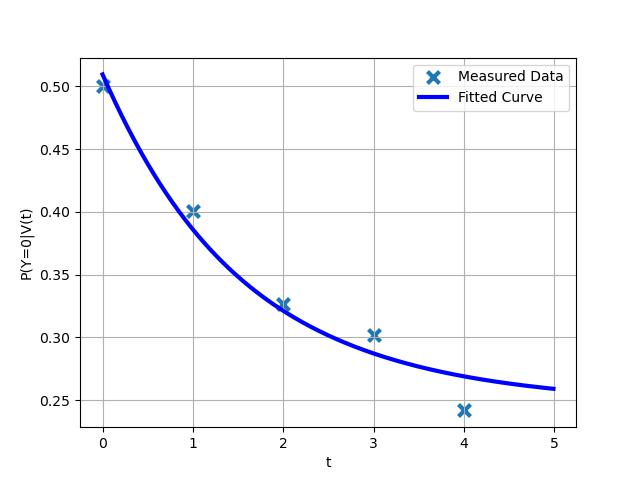
\includegraphics[width=0.45\textwidth]{逻辑回归_雌性概率.jpg}}			  % 子图1的图片宽度 不能空行
	\subfigure[$P\left( \left. Y=0 \right|V\left( t \right) \right)$]{				% 图片2
		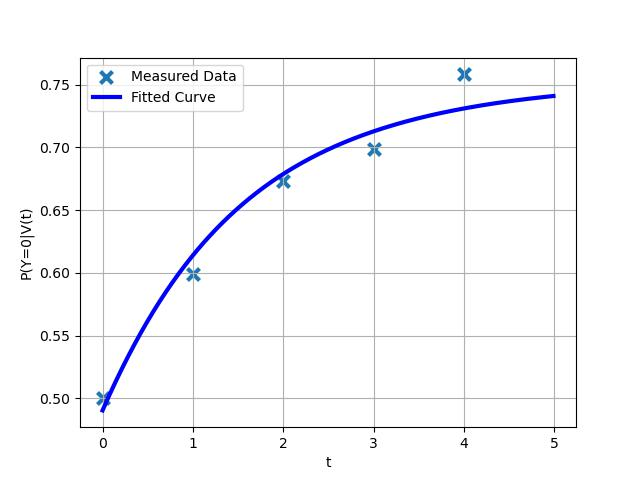
\includegraphics[width=0.45\textwidth]{逻辑回归_雄性概率.jpg}}
	
	\caption{Model and Data Fitting} % 图片标题 
\end{figure}

The diagram presented earlier illustrates how the gathered data is utilized to calibrate our model.
\subsubsection{The Growth Model of Population in A Given Area}

Now that we have looked at the growth model of individuals in a population, we will look at the growth model of the population as a whole.  The \textbf{traditional Logistic model} has given us the direction to solve this kind of problem, but due to the limitation of practical problems, we need to revise it.

The total number of individuals in the lamprey population is now divided into the sum of males and females, as indicated by the following mathematical expression:
\begin{equation}
	N=M+F
\end{equation}
where:
\begin{itemize}
	\setlength{\parsep}{0ex} %段落间距
	\setlength{\topsep}{2ex} %列表到上下文的垂直距离
	\setlength{\itemsep}{1ex} %条目间距
	\item $N$  is the total number of individuals in the population.
	\item $M$  is the total number of males in the population.
	\item $F$ is the total number of females in the population.
\end{itemize}

Next, we separate the male and female, and modify the traditional Logistic model to list the following equation:
	\begin{equation}
		\begin{cases}
			\frac{dM}{dt}=e_{i}c_i\phi _iF-\gamma \left( F+M \right) ^2\\
			\frac{dF}{dt}=e_{i}\left( 1-c_i \right) \phi _iF-\gamma \left( F+M \right) ^2\\
			\frac{dM}{dt}+\frac{dF}{dt}=\frac{dN}{dt}\\
		\end{cases}
	\end{equation}
where:
\begin{itemize}
	\setlength{\parsep}{0ex} %段落间距
	\setlength{\topsep}{2ex} %列表到上下文的垂直距离
	\setlength{\itemsep}{1ex} %条目间距
	\item $\phi_{i}$ is the number of eggs that hatch successfully\upcite{3,4}.
	\item $c_{i}$  is the proportion of eggs that develop into males.
	\item $\gamma$ is the parameter used to modify the equation.This parameter is mainly demermined by intrinsic growth rate and environmental capacity. 
	\item  $e_{i}$ is larval survival rate.
\end{itemize}
\begin{figure}[H]  %h此处,t页顶,b页底,p独立一页,浮动体出现的位置
	\centering  %图表居中
	\includegraphics[width=.8\textwidth]{拟合.png} %图片的名称或者路径之中有空格会出问题 
	\caption{Model and Data Fitting}
\end{figure}

As shown in the figure above, we use the data we have collected to fit our model。
\subsection{Model II: Interaction Model between Lampreys and External Environment}
\subsubsection{Predation Model of Lampreys}
Now we consider lampreys in an ecosystem.  According to the assumption 5, lampreys have almost no natural enemies and competitors in the ecosystem.
 Therefore, we will solely focus on their predatory relationships with other species.  We define $x$ as a function of the prey population size of lampreys and time $t$, which can be determined using the \textbf{Lotka-Volterra equation},the specific equation is as follows:
\begin{equation}
	\frac{dX}{dt}=\alpha\cdot X-\delta \cdot X\cdot N
\end{equation}
where:
\begin{itemize}
	\setlength{\parsep}{0ex} %段落间距
	\setlength{\topsep}{2ex} %列表到上下文的垂直距离
	\setlength{\itemsep}{1ex} %条目间距
	\item $X$ is the total number of individuals in the prey population.
	\item $N$ is the total number of lampreys in the population.
	\item $\alpha$  is the natural growth rate of the prey population.
	\item $\delta $ is the percentage of the total prey that is hunted.
\end{itemize}

\subsubsection{Lamprey-Environment Interaction Model}
The environmental impacts of lampreys mainly include species diversity $y_{1}$, trophic status index $y_{2}$ , species richness $y_{3}$ and species uniformity $y_{4}$. In order to facilitate the study, we mainly focus on the sex ratio $x_{1}$, growth rate of lampreys $x_{2}$, and population size $x_{3}$.In order to facilitate our research on the interaction system between the population of lampreys $N$, and the subsystems of resources and environment, we have developed an \textbf{evaluation system }denoted as $f(L)$ for lampreys and an evaluation system denoted as $f(R)$ for resources and environment.We have the following equation:
\begin{equation}
	\begin{cases}
		f\left( N \right) =a_1x_1+a_2x_2+a_3x_3\\
		f\left( R \right) =b_1y_1+b_2y_2+b_3y_3+b_{4}y_{4}\\
	\end{cases}
\end{equation}
where:
\begin{itemize}
	\setlength{\parsep}{0ex} %段落间距
	\setlength{\topsep}{2ex} %列表到上下文的垂直距离
	\setlength{\itemsep}{1ex} %条目间距
	\item $a_{i}$ and $ b_{j}$ ($i=1,2,3 $, $j=1,2,3,4$) represent the weight of each corresponding element in the whole.
\end{itemize}

\begin{figure}[H] %h此处,t页顶,b页底,p独立一页,浮动体出现的位置
	\centering  %图表居中
	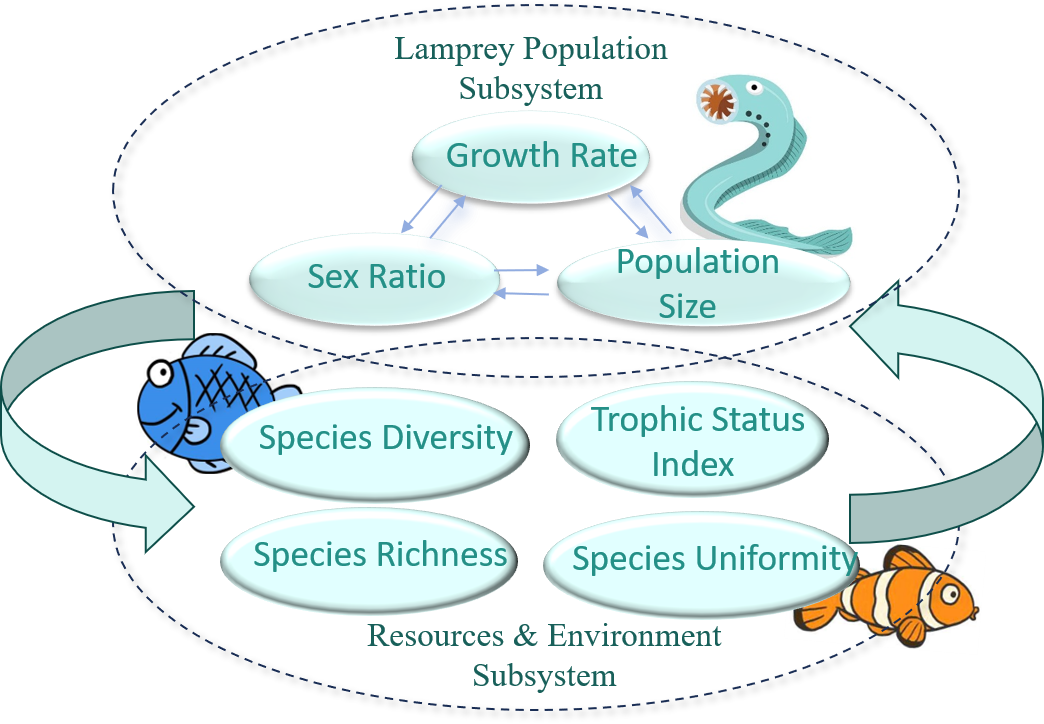
\includegraphics[width=.6\textwidth]{图片1.png} %图片的名称或者路径之中有空格会出问题 
	\caption{The Fluctuations in  Lamprey Populations and Prey Numbers in Low Sex Ratio}
\end{figure}
After defining these main parameters, we also need to define\textbf{ interaction degree}  $\varepsilon$\upcite{5} to represent the degree of interaction between the two subsystems of lamprey population $N$ and resource environment,the specific expression is as follows:
\begin{equation}
	\varepsilon =\mathrm{arc}\tan \frac{f\left( L \right)}{f\left( R \right)}
\end{equation}

After standardizing the data from multiple systems in the Great Lakes and evaluating the fitting parameters, we obtained diverse outcomes that can be roughly categorized based on the $\varepsilon$ value.The resulting interaction ranges and categories are listed in the Table 3 :

\begin{table}[htbp]
	\begin{center}
		\caption{Interaction Range and Classification}
		\resizebox{\textwidth}{!}
		{\begin{tabular}{c c}
				\toprule[2pt]
				\multicolumn{1}{m{5cm}}{\centering \textbf{Interaction Range/Degree}}
				&\multicolumn{1}{m{10cm}}{\centering \textbf {Classification} }\\ %m后面是列宽
				\midrule
				$0<\varepsilon<35$& No Significant Interaction\\
				$35<\varepsilon<75$ &Benign Interaction\\
				$75<\varepsilon<90$ & Malignant Interaction \\
				\bottomrule[2pt]
		\end{tabular}}
	\end{center}
\end{table}
\vspace{-0.8cm}
\subsection{Model III : Host-Parasite Model}
Based on model \textbf{Lotka-Volterra }, we use it to describe the relationship between host and parasite.The specific equation is as follows:
\begin{equation}
	\frac{dI}{dt}=r\cdot q\cdot J\cdot I-h\cdot I
\end{equation}

where:
\begin{itemize}
	\setlength{\parsep}{0ex} %段落间距
	\setlength{\topsep}{2ex} %列表到上下文的垂直距离
	\setlength{\itemsep}{1ex} %条目间距
	\item $r$ is the number of parasites in each host.
	\item $q$ is the ratio of the number of hosts infected by parasites to the total population.
	\item $J$ is the number of hosts.
	\item $I$ is the number of parasites.
	\item $h$ is the natural mortality rate of parasites
\end{itemize}

\subsection{Reasonable Estimation of Essential Parameters}
\subsubsection{Estimation of Growth Rate Parameters $k$}
It is difficult to find direct data to support the specific value of  $k$ corresponding to lampreys, but we can fit the corresponding parameters by nonlinear least square method. At this point we can get an estimate of $k$:
\begin{equation}
	k=0.5699
\end{equation}

In order to verify the accuracy of the estimated parameters, we analyzed them by means of mean absolute error (MAE) and root mean square error (RMSE) respectively. The corresponding formulas are as follows:
\begin{equation}
	MAE=\frac{1}{m}\sum_{i=1}^m{|y_i-\hat{y}_i}|
\end{equation}
\begin{equation}
RMSE=\sqrt{\frac{\sum_{i=1}^m{\left( y_i-\hat{y}_i \right) ^2}}{m}}
\end{equation}
where:
\begin{itemize}
	\setlength{\parsep}{0ex} %段落间距
	\setlength{\topsep}{2ex} %列表到上下文的垂直距离
	\setlength{\itemsep}{1ex} %条目间距
	\item $m$ is the total number of samples.
	\item $y_{i}$ is the actual value of the sample.
	\item $\hat{y}_i$ is the sample value predicted by the model.
\end{itemize}

Then we can get the corresponding MAE and RMSE:
\begin{equation}
	\begin{cases}
		MAE=8.5400\\
		RMSE=9.4373\\
	\end{cases}
\end{equation}

The calculation results show that the fitted $k$ has a high accuracy.
\subsubsection{Estimation of Logistic Regression Parameters $\beta_{0}$ and $\beta_{1}$}
For a binary classification problem with only male and female as mentioned above, we apply logistic regression model, but at the same time introduce two important logistic regression parameters $\beta_{0}$ and $\beta_{1}$, the values of these two important parameters cannot be obtained through theoretical deduction, so we search relevant data and apply mode to fill a small number of missing values in their data. After the unreasonable value is deleted, we use the nonlinear least square method to fit the processed data to estimate the two parameters, and finally get the following values:
\begin{equation}
	\begin{cases}
		\beta _0=1.1184\\
		\beta _1=-0.0107\\
	\end{cases}
\end{equation}

And again, we're going to do an error analysis:
\begin{equation}
	\begin{cases}
		MAE=0.0143\\
		RMSE=0.0160\\
	\end{cases}
\end{equation}

The calculation results show that our fitting results are good.
\subsubsection{Estimation of $\phi_{i}$ and $e_{i}$}

Since these two parameters are related to the actual situation of the ecological environment, we discussed the actual situation of the Great Lakes respectively. The specific parameters and error analysis are listed in the  Table 4:

\begin{table}[H]
	\begin{center}
		\caption{Error Analysis and Parameter Estimation}
		\resizebox{\textwidth}{!}
		{\begin{tabular}{c c c c c}
				\toprule[2pt]
		\multicolumn{1}{m{3cm}}{\centering \textbf{Lake Name}}	&\multicolumn{1}{m{3cm}}{\centering $\phi_{i}$ }&\multicolumn{1}{m{3cm}}{\centering $e_{i}$ }&\multicolumn{1}{m{3cm}}{\centering $MAE$ }&\multicolumn{1}{m{3cm}}{\centering $RMSE$ }\\
				\midrule
				Superior & 0.0019 &0.0058 &0.3947& 0.5829\\
				Erie & 0.0013 &0.0970 & 2.2922 & 4.5621 \\
				Huron & 0.0003 &0.0003 & 0.1988 & 0.2547\\
				Miichigan & 0.0008 & 0.0021 & 0.2199 & 0.2565\\
				Ontario & 0.0146 &0.0005 &0.2168 &0.2925\\
				\bottomrule[2pt]
		\end{tabular}}
	\end{center}
\end{table}
\vspace{-0.8cm}
On the whole, our model has a good fitting result to the actual data.
\section{Model Computed and Results Analysis}
\subsection{The Impact of Sex Ratios on Ecosystems}
\subsubsection{Effects on Species}
Now, in order to solve the effect of the male and female population of lampreys on the population of other species, we apply the \textbf{Sex Sex Determination Model} of lampreys in Model I.From the previously deduced model relationship, we have:
\begin{equation}
	1-c_i=P\left( \left. Y=1 \right|V\left( t \right) \right) =\frac{e^{\beta _0+\beta _1\cdot V\left( t \right)}}{1+e^{\beta _0+\beta _1\cdot V\left( t \right)}}
\end{equation}

Then, from formulas (6) and (17), we can get the following equations:
	\begin{equation}
		\begin{cases}
			1-c_i=\frac{e^{\beta _0+\beta _1\cdot V\left( t \right)}}{1+e^{\beta _0+\beta _1\cdot V\left( t \right)}}\\
			\frac{dM}{dt}=e_{i}c_i\phi _iF-\gamma \left( F+M \right) ^2\\
			\frac{dF}{dt}=e_{i}\left( 1-c_i \right) \phi _iF-\gamma \left( F+M \right) ^2\\
			\frac{dM}{dt}+\frac{dF}{dt}=\frac{dN}{dt}\\
		\end{cases}
	\end{equation}

At this time, we add the consideration of the population number formula of prey animals, apply the mathematical model to simulate, and get the following image:

\begin{figure}[H]  %h此处,t页顶,b页底,p独立一页,浮动体出现的位置
	\centering  %图表居中
	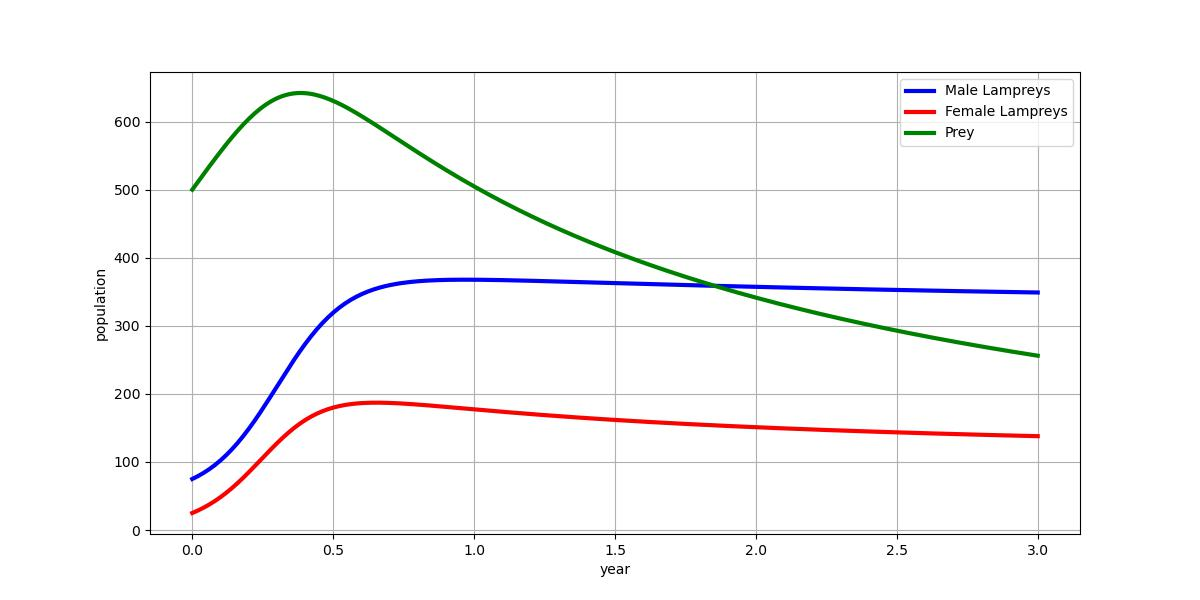
\includegraphics[width=.6\textwidth]{test(1)(1).jpg} %图片的名称或者路径之中有空格会出问题 
	\caption{Simulation of Lampreys and Their Relationships with Other Species}
\end{figure}
\vspace{-0.8cm}
From the Figure 7, we can intuitively draw the following conclusions:

\textbf{Conclusion}:On the whole, the population of lampreys showed an upward trend, while the prey population showed a downward trend.Finally, the three tend to stabilize.

\subsubsection{Effects on Environment}
We applied Model II to discuss the impact of the sex ratio of lampreys on the environment. After searching the four evaluation indexes of resources and environment on Google Scholar, we found that the keyword \textbf{species diversity} had 201,000 indexes, \textbf{nutritional status} had about 260,000 indexes, and\textbf{ species richness} and \textbf{species uniformity} were 125,000 and 56,500, respectively. The same can be said for the weight of lampreys species and from this data, so we can estimate the relative weight of each indicator .

In order to solve the dimensional inconsistency brought by multivariate data, we need to standardize the data processing, the specific method is as follows:

For positive indices,we have
\begin{equation}
	X_i=\frac{x_i-x_{\min}}{x_{\max}-x_{\min}}
\end{equation}

For  negative indices,we have
\begin{equation}
	X_i=\frac{x_{\max}-x_{i}}{x_{\max}-x_{\min}}
\end{equation}
where,$X_{i} $ is the standardized value of indicator $ i$, $x_{i} $ is the initial value of indicator $i$, $x_{\max}$ and $x_{\min}$ are the maximum and minimum values respectively.

Then we can get a standardized equation:
	\begin{equation}
		\begin{cases}
			f\left( N \right) =0.15586X_1+0.6822X_2+0.1592X_3\\
			f\left( R \right) =0.3128Y_1+0.4047Y_2+0.1946Y_3+0.0882Y_{4}\\
		\end{cases}
	\end{equation}
After bringing in the corresponding data of the Great Lakes, we can get the values corresponding to different sex ratio interaction degrees  $\varepsilon$. At this time, we find that the value of $\varepsilon$ is a malignant interaction between the male ratio of 48$\% $ and 63$\%$, and a benign interaction when the male ratio exceeds 63$\%$.
\subsection{The Strengths and Weaknesses of Lampreys Populations}
\subsubsection{The Strengths of Lampreys Populations}
By considering the \textbf{Sex Determination Model} and\textbf{ Predation Model of Lampreys}, we measure the value of food availability $ R $ through the \textbf{ Predation Model of Lampreys}. With the change of $R$, we obtain the change wave equation (4) of $V (t)$, and thus obtain the probability equation (3) of sex-sex transition $c_{i}$ and $1-c_{i}$ through\textbf{ Logistic Regression}, which we bring into equation (6). Combined with equation (4), by simulating the model, the images of the changes in the number of male and female lampreys and the number of prey are obtained in Figure 8:
\vspace{-0.4cm}
\begin{figure}[H] %h此处,t页顶,b页底,p独立一页,浮动体出现的位置
	\centering  %图表居中
	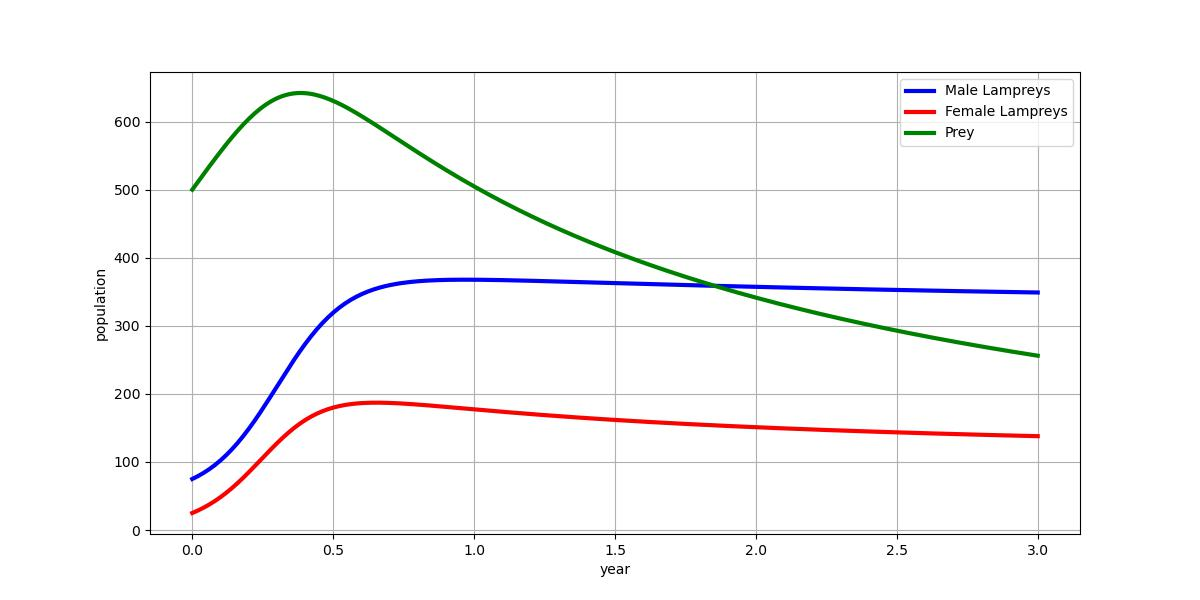
\includegraphics[width=.6\textwidth]{test(1)(1).jpg} %图片的名称或者路径之中有空格会出问题 
	\caption{The Fluctuations in Male and Female Lamprey Populations and Prey Numbers}
\end{figure}
\vspace{-0.8cm}
We can see that when food is sufficient, the number of males and females of lampreys increases, but with the increase of the number of males and females of lampreys, the availability of food gradually decreases.When food is scarce, the growth rate of lampreys decreases, which changes the sex ratio and further changes the rate of population growth, thereby controlling the population and stabilizing the number of prey and the number of males and females.We came to the following conclusion:

\textbf{Conclusion:}The\textbf{ advantage} of lampreys is that when food is reduced, lampreys can control their own growth rate by controlling the sex ratio, so as to adapt to the food shortage environment and keep the population basically stable.

\subsubsection{The Weaknesses of Lampreys Populations}

When the male ratio is low, the number of the species declines, and the number of prey increases substantially with the reduction of predators.  Although abundant food is obtained, rapid reproduction is difficult due to the imbalance of the sex ratio.  We set the initial male ratio far from the optimal sex ratio and the food quantity is sufficient, and we can see that the number of species cannot increase rapidly within three years from Figure 9:

\begin{figure}[H] %h此处,t页顶,b页底,p独立一页,浮动体出现的位置
	\centering  %图表居中
	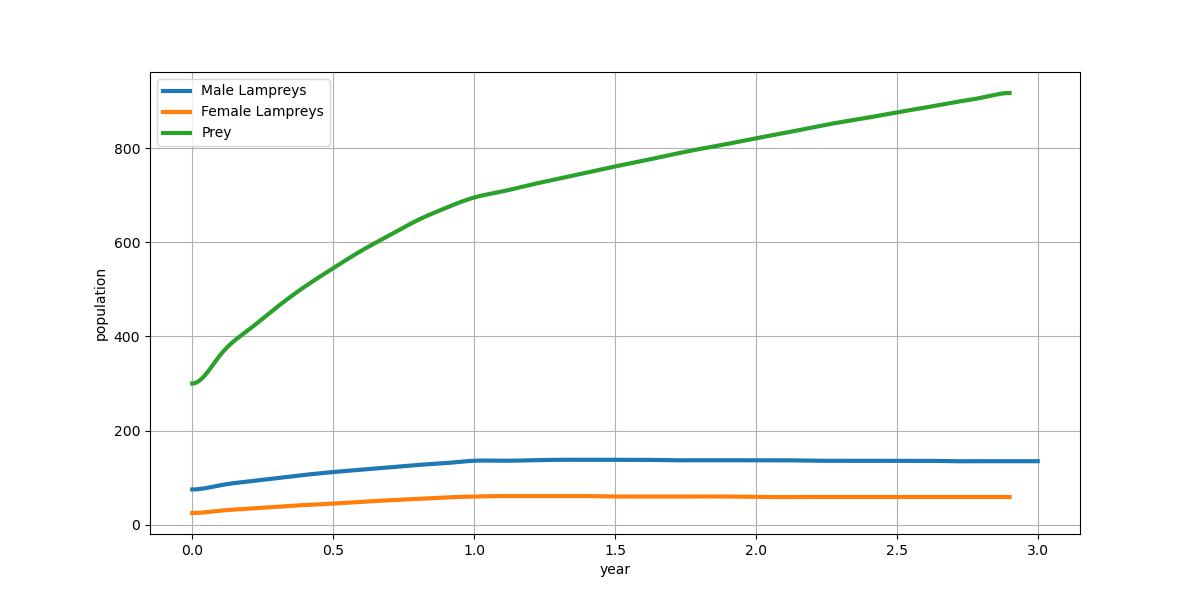
\includegraphics[width=.6\textwidth]{模拟2.jpg} %图片的名称或者路径之中有空格会出问题 
	\caption{The Fluctuations in  Lamprey Populations and Prey Numbers in Low Sex Ratio}
\end{figure}
\vspace{-0.8cm}
From the image, we can easily draw the following conclusion: 

\textbf{Conclusion:}The \textbf{disadvantage} of lampreys population is that when food changes from scarcity to abundance, its growth is affected by the imbalance of sex ratio, and it is difficult to grow and reproduce quickly.
\subsection{The Impact of Sex Ratios on Ecosystem Stability}
\subsubsection{Ecological Environment Stability}
%Some indicators are needed to assess the stability of the ecological environment: Common features include ecosystem diversity, richness and ecosystem function.  We used the \textbf{Lamprey-Environment Interaction Model} of Model II to assess the environment's river bed structure, water body nutrition and species diversity respectively.  Taking Lake Michigan as an example, we saw that the data of lampreys in Lake Michigan declined under control and species diversity remained stable in 2016 through the data report of the Great Lakes.  The eutrophication of water body is decreased.We defined the evaluation system to give score evaluation, and finally got the interaction degree of 83.498, which was benign coupling and in line with the given data conditions. The other calculations basically show a good degree of interaction, and we can know that lampreys are conducive to ecological stability.

We apply the evaluation model of Model II, according to
\begin{equation}
	\begin{cases}
		f\left( N \right) =0.15586X_1+0.6822X_2+0.0.1592X_3\\
		f\left( R \right) =0.3128Y_1+0.4047Y_2+0.1946Y_3+0.0882Y_{4}\\
	\end{cases}
\end{equation}
The growth rate is changed in order to examine the impact on sexual transformation and its subsequent influence on interaction patterns.Using the Lake Michigan data of 2016, 2017, 2018, 2019 and 2021, we substituted the mathematical model to obtain the relationship between sex ratio and interaction degree as follows:
\vspace{-0.5cm}
\begin{figure}[H] %h此处,t页顶,b页底,p独立一页,浮动体出现的位置
	\centering  %图表居中
	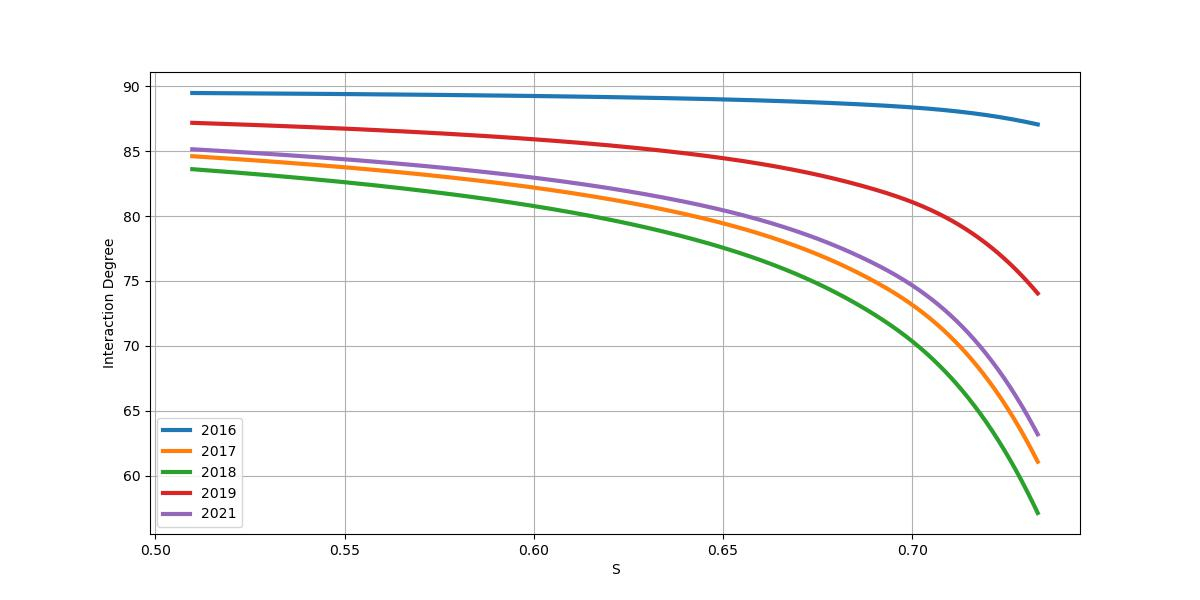
\includegraphics[width=.6\textwidth]{5 (1).jpg} %图片的名称或者路径之中有空格会出问题 
	\caption{The Relationship between Sex Ratio and Interaction Degree}
\end{figure}
\vspace{-0.8cm}
We found that when the sex ratio is 50$\%$, the interaction degree is \textbf{85.84}, which is a malignant interaction, but with the increase of the sex ratio, the interaction degree to the environment reaches the minimum of \textbf{67.96}. According to the evaluation system, it is a benign coupling. Therefore, we know that as the sex ratio approaches 50\textbf{\%}, the interaction degree increases to the maximum. It is harmful to the stability of the environment.

\subsubsection{Species Stability}
We add some perturbations to the prey population in the model, so that the prey population suddenly drops, and we find that lampreys change their sex ratio because the lack of food affects their growth rate, so that the prey population increases in the subsequent time, and the populations return to normal.
\begin{figure}[H] %h此处,t页顶,b页底,p独立一页,浮动体出现的位置
	\centering  %图表居中
	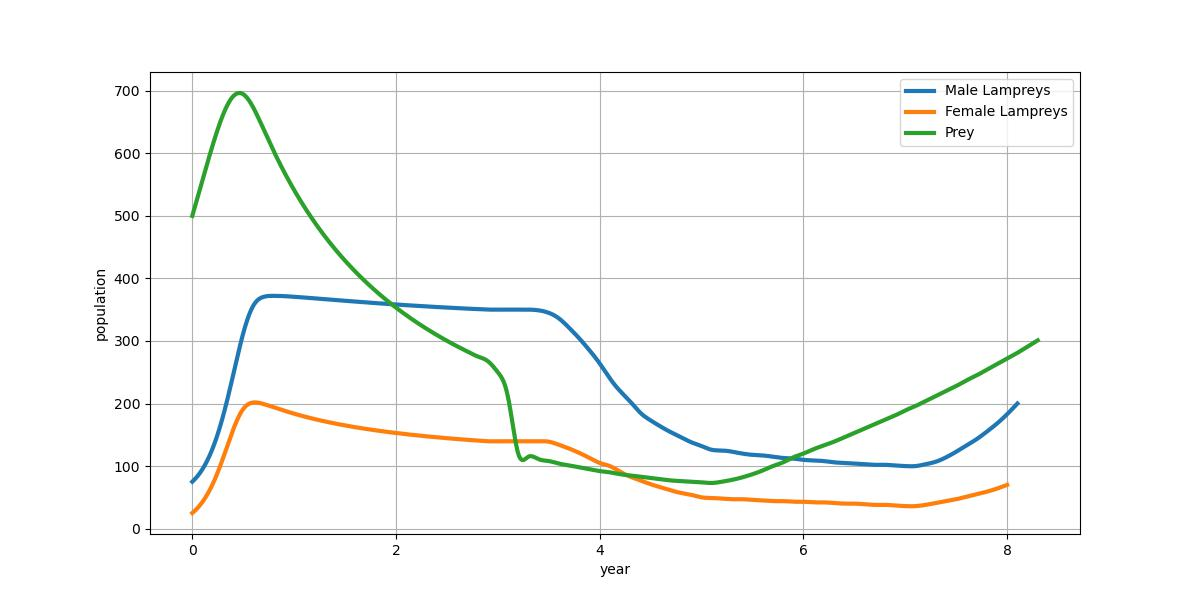
\includegraphics[width=.6\textwidth]{模拟 (1).jpg} %图片的名称或者路径之中有空格会出问题 
	\caption{Simulation of population changes during food shocks}
\end{figure}
\subsection{The Impact of Ecosystems On Parasites}
We now consider the relationship between lampreys and parasites, introducing \textbf{Host-Parasite Model}:
\begin{equation}
		\frac{dP}{dt}=r\cdot q\cdot J\cdot I-h\cdot I
\end{equation}

Since the main target of bottom-bottom parasites is fish, and the main prey of lampreys is also fish, the number of hosts $J$ equals to the number of prey $X$.

Combine the \textbf{Sex Determination Model} of Model I
\begin{equation}
	P\left( \left. Y=1 \right|V\left( t \right) \right) =\frac{e^{\beta _0+\beta _1\cdot V\left( t \right)}}{1+e^{\beta _0+\beta _1\cdot V\left( t \right)}}
\end{equation}

 with the\textbf{ Predation Model} of Model II
 \begin{equation}
 	\frac{dX}{dt}=\alpha\cdot X-\delta \cdot X\cdot N
 \end{equation}
 
The simulation results of our model are as follows:
 \begin{figure}[H] %h此处,t页顶,b页底,p独立一页,浮动体出现的位置
 	\centering  %图表居中
 	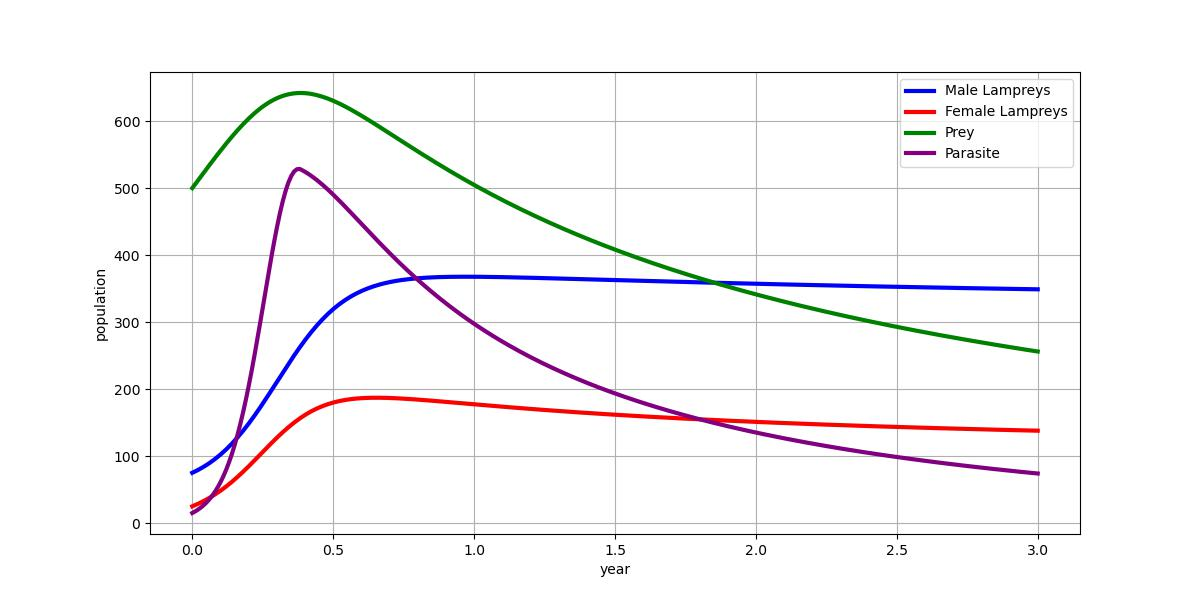
\includegraphics[width=.6\textwidth]{test(2).jpg} %图片的名称或者路径之中有空格会出问题 
 	\caption{The Fluctuations in Lamprey Populations and Prey Numbers after parasite introduction}
 \end{figure}
 \vspace{-0.4cm}
 From the Figure 12, we can see: when the number of lampreys was low, the parasite multiplied rapidly in the fish and the number increased sharply, but with the increase of the number of lampreys, the number of predation on fish also increased, making the number of fish decline, reducing the number of parasite hosts, causing a large number of parasites to die, and finally with the stability of the number of lampreys species and prey, the parasite number also stabilized.  So we come to the following conclusion:
 
 \textbf{Conclusion:}As the number of lampreys increased, the number of parasites decreased and both eventually leveled off, and lampreys don't prey on parasites, so we know that\textbf{ the relationship is competitive} and it can not offer advantage to others in the ecosystem..

\section{Sensitivity Analysis}
In \textbf{Sec.5}, we build three large models, and in\textbf{ Sec.5.4}, we give reasonable estimates for some important parameters among them. However, we cannot estimate some parameters, which can only be obtained by searching the literature. So we need to perform sensitivity analysis on these parameters.

The first is the maximum attainable length of an individual organism $L_{\infty}$.By adjusting the value of $L_{\infty}$, we get the sensitivity analysis curve, which is as follows:
\vspace{-5cm}
\begin{figure}[H]  %h此处,t页顶,b页底,p独立一页,浮动体出现的位置
	\centering  %图表居中
	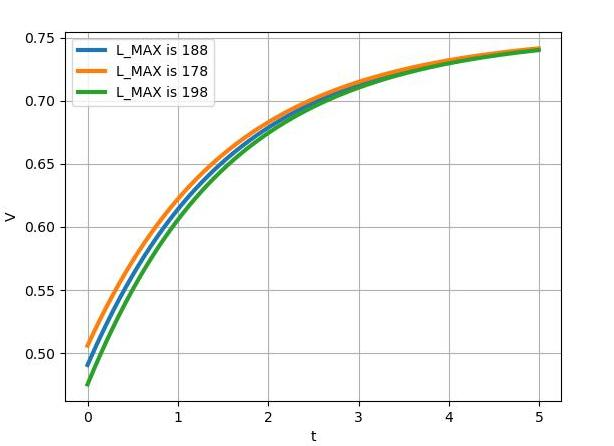
\includegraphics[width=.6\textwidth]{灵敏度分析.jpg} %图片的名称或者路径之中有空格会出问题 
	\caption{The Sensitivity Analysis of $L_{\infty}$}
\end{figure}

Then, we analyze the sensitivity of $\phi_{i}$ ,which is the number of eggs that hatch successfully.
\vspace{-0.5cm}
\begin{figure}[H]  %h此处,t页顶,b页底,p独立一页,浮动体出现的位置
	\centering  %图表居中
	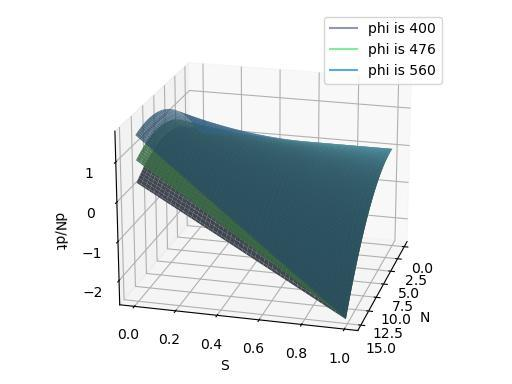
\includegraphics[width=.6\textwidth]{灵敏度分析1 (3).jpg} %图片的名称或者路径之中有空格会出问题 
	\caption{The Sensitivity Analysis of $\phi_{i}$}
\end{figure}
\vspace{-0.6cm}
Lastly, we analyze the sensitivity of $\alpha$ (The natural growth rate of the prey population) and $\delta$ (The percentage of the total prey that is hunted).
\vspace{-0.3cm}
\begin{figure}[H]
	\centering    
	\subfigure[The Sensitivity of $\alpha$]{				% 图片1([]内为子图标题)						
		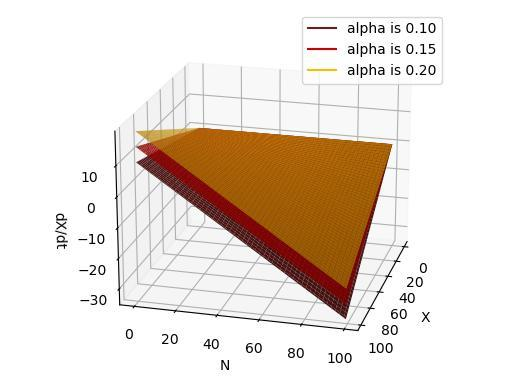
\includegraphics[width=0.4\textwidth]{灵敏度分析2.jpg}}			  % 子图1的图片宽度 不能空行
	\subfigure[The Sensitivity of $\delta$]{				% 图片2
		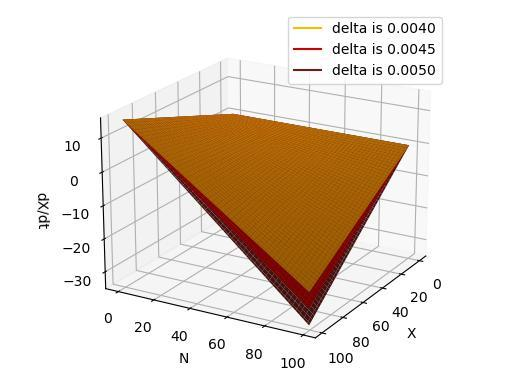
\includegraphics[width=0.4\textwidth]{灵敏度分析3.jpg}}
	
	\caption{Model and Data Fitting} % 图片标题 
\end{figure}
\vspace{-0.7cm}
Through proper adjustment of parameters, we found that the trend of model change is basically consistent, so our model has a good stability.
\section{Model Evaluation}
\subsection{Strengths}
\begin{itemize}
	\setlength{\parsep}{0ex} %段落间距
	\setlength{\topsep}{2ex} %列表到上下文的垂直距离
	\setlength{\itemsep}{1ex} %条目间距
	\item Our  \textbf{Growth Model  of An Individual}  is universal, and in addition to the actual growth of lampreys, we can also simulate the actual growth of other egg-laying creatures.
	\item In our \textbf{Sex Determination Model}, we can refer to it for simulating the relationship between the male sex ratio and the individual growth rate of any species population, since we do not restrict it.
	\item The \textbf{interaction degree}   we define is an intuitive representation of the degree of interaction between a species and its environment. It can intuitively represent the impact of species on the stability of ecological environment.
\end{itemize}
\subsection{Weaknesses }
\begin{itemize}
	\setlength{\parsep}{0ex} %段落间距
	\setlength{\topsep}{2ex} %列表到上下文的垂直距离
	\setlength{\itemsep}{1ex} %条目间距
	\item Although we use a large number of parameters for the model to represent the flexibility of the model, some parameters cannot be accurately calculated and can only be queried by reference. But we have fully verified the correctness of its parameters.
	\item Our main consideration for the survival resources of lampreys is fish resources, which is somewhat deviated from the actual situation.
\end{itemize}
\section{Conclusion}
\begin{enumerate}[\bfseries \textit{Task} 1:]
	\item For the sake of discussion, we categorize the problem into the impact of Lampreys on the environment and the impact of Lampreys on other species in the ecosystem. Based on Sex Determination Model and The Growth Model of Model I and Lamprey-Environment Interaction Modelof model II, we derive: When the male sex ratio of lampreys is between 48$\%$ and 63$\%$, the interaction with the ecosystem is malignant .
	\item Based on the Sex Determination Model  of Model Iand Predation Model of Lampreysof Model II, we obtained through computer simulation that lampreys had the advantage that they could control the sex ratio to maintain the stability of the population, and the disadvantage was that they could not reproduce quickly when the male and female ratio was too low.
	\item For the convenience of evaluation, we classified the problem into the impact of lampreys on environmental stability and the impact of lampreys on the stability of other species in the ecosystem.  The calculation results showed that it was beneficial to the stability of the ecological environment and the stability of other species in the ecosystem ,which is in the right sex ratio.
	\item After the introduction of the parasite, we based on the Sex Determination Model, Predation Model and Host-Parasite Model, through computer simulation, we got a competitive relationship between the parasite and the lampreys.It follows that  an ecosystem with variable sex ratios in the lamprey population can not offer advantage to others in the ecosystem.
\end{enumerate}

% 参考文献,此处以 MLA 引用格式为例
\clearpage   %另起一页继续写。这时,你最好使用“\clearpage” 
\begin{thebibliography}{99}
    \bibitem{1} Great Lakes Fishery Commission http://www.glfc.org/pulse-on-science-making-the-best.php
	\bibitem{2} JIM HONE, TIM H.Climate, food, density and wildlife population growth rate.Journal of Animal Ecology,2007,76(2):361-367
	\bibitem{3} Patrick J. Manion,Lee H. Hanson.Spawning Behavior and Fecundity of Lampreys from the Upper Three Great Lakes.Canadian Journal of Fisheries and Aquatic Sciences ,November ,1980
	\bibitem{4} Michael J. Hansen and Michael J. Hansen etc. Population ecology of the sea lamprey (Petromyzon marinus) as an invasive species in the Laurentian Great Lakes and an imperiled species in Europe.Reviews in Fish Biology and Fisheries,2016,26(6):509-535
	\bibitem{5} Cong L J W C T. Study on the Spatial Coupling Analysis Method of Human-land 
	Relationship in Nature Reserves——A Case Study of Tianmushan Nature Reserve [J]. 
	Chinese Landscape Architecture, 2022, 38(05): 74-79

\end{thebibliography}
% \includepdf[pages={1,2}]{Memo.pdf} 
\clearpage

\section*{Report on Use of AI}
Open AI ChatGPT(Nov 5,2023 version,ChatGPT-4)
\begin{enumerate}[\bfseries \textit{Query} 1:]
	\item \textbf{What are the predators of lampreys?}\\
	\textbf{\textit{Output:}}Lampreys may become food for a variety of predators at different stages of their life cycle. In the larval stage, they may be preyed upon by some bottom-dwelling fish, birds, and other large invertebrates. Adult lampreys have fewer predators due to their parasitic lifestyle, but can still be preyed upon by some large fish and Marine mammals. Specific predators vary depending on their environment and geographic location.
	\item \textbf{How long do lampreys live?}\\
	\textbf{\textit{Output:}}The lifespan of lampreys varies according to different stages of their life cycle. The larval stage can last for about three to seven years, but as adults, Lampreys enter the breeding period, when they leave their host and go up to fresh water to breed. Adult lampreys usually die after breeding, meaning that their life ends after they complete one breeding cycle, which usually lasts no more than a year. So the whole life cycle is about four to eight years.
	\item \textbf{How is the stability of an ecosystem measured?}\\
	\textbf{\textit{Output:}}The stability of an ecosystem refers to its ability to maintain its structure and function in the face of external disturbances such as climate change, invasive species, human activities, etc. Measuring ecosystem stability is a complex task because it involves multiple ecological processes and attributes. In general, ecosystem stability can be assessed from the following dimensions:
	\begin{enumerate}
		\item Resistance: The ability of an ecosystem to maintain its original state in the face of short-term environmental changes or disturbances. Highly resistant ecosystems can remain relatively unchanged after disturbance.
		\item Resilience: The ability and speed of an ecosystem to return to its original state or function after being disturbed. Resilient ecosystems are able to recover from disturbances in a relatively short time.
		\item Stability: Usually refers to the magnitude of changes in ecological processes and service functions of an ecosystem in the face of disturbances. Low variability means high stability.
		\item Persistence: The ability of an ecosystem to maintain its species diversity and ecological structure without long-term disturbance.		
	\end{enumerate}
	
\end{enumerate}
\setcounter{page}{20}

\end{document}  % 结束